\documentclass{article}
% ICLR 2027 style not yet released (as of 2026-07). Using iclr2026 style;
% swap the two lines below + .bst when the official 2027 kit ships.
\usepackage{iclr2026_conference,times}
\input{math_commands.tex}

\usepackage{hyperref}
\usepackage{url}
\usepackage{graphicx}
\usepackage{booktabs}
\usepackage{multirow}
\usepackage{amsmath,amssymb}
\usepackage{subcaption}
\usepackage{tikz}
\usetikzlibrary{arrows.meta,positioning}

\title{EpiSpace: Counterfactual Episode Families\\
for Systematic Spatial Composition}

% Anonymous by default; uncomment for camera-ready.
% \iclrfinalcopy

\author{Anonymous authors\\
\texttt{anonymous}}

\begin{document}

\input{generated/dataset_stats}
\maketitle

\begin{abstract}
Spatial QA accuracy alone cannot distinguish a reusable scene model from a
question-specific shortcut.  We ask a controlled question: under identical
selected facts and, in the stricter regime, matched image/pixel exposure, does
\emph{observe-first, read-many}
supervision improve unseen compositions over isolated QA?  We introduce
\textbf{EpiSpace}, a geometry-to-episode compiler whose basic unit is a
counterfactual sibling family.  Siblings share a scene and latent fact while a
single evidence or reference-frame intervention requires the answer to change,
remain valid, or become unknown.  Typed answer-free programs define a
signature-disjoint composition split; geometry remains hidden and is used only
to construct and independently replay certificates.  The frozen pilot audits
\EpiPlannedJobs{} simulator jobs, retains \EpiStrictBundles{} strict bundles
over \EpiScenes{} scenes, and extracts \EpiSourceViews{} raw RGB views from
\EpiSourceTrajectories{} write trajectories.  It compiles
\EpiCompiledQuestions{} questions and \EpiConsistencyFamilies{} complete
families---\EpiEvidenceFamilies{} evidence triples, \EpiClaimFamilies{} claim
pairs, and \EpiFrameFamilies{} frame-equivariant pairs.  The release exports
\EpiSupervisedFacts{} exactly paired training facts and a
\EpiCoreBenchmarkRecords{}-item core benchmark containing
\EpiFamilyBenchmarkGroups{} scene-disjoint families and
\EpiCompositionRecords{} held-out-program items.  All
\EpiReplayedCertificates{} targets replay from source geometry; raw-RGB purity,
family completeness, input--target functionality, split locks, and target-view
hash isolation pass.  We also release deterministic fact-matched and
image-occurrence-matched schedules and define accuracy-conditioned evidence
sensitivity, which cannot be maximized by always abstaining.  This paper
reports a validated data asset and a falsifiable training protocol; image and
pixel exposure are controlled, but text tokens, FLOPs, and wall-clock compute
are not matched.  No model improvement is claimed before the frozen comparison
is run.
\end{abstract}

\section{Introduction}
\label{sec:intro}

Multimodal large language models (MLLMs) can recognize furniture yet fail when
the answer requires joining separated views, changing reference frames,
remembering an object that left view, or distinguishing \emph{unseen} from
\emph{absent}.  VSI-Bench, MindCube, MMSI-Bench, and ViewSpatial-Bench expose
complementary versions of this gap~\citep{yang2024thinking,yin2025mindcube,
yang2025mmsi,li2025viewspatial}.  Large instruction collections such as
SenseNova-SI broaden coverage, but their analyses also show shortcut
sensitivity and mixed gains from textual chain-of-thought
recipes~\citep{cai2025sensenova}.  The remaining issue is not simply how many
spatial answers a model sees, but which computation its supervision makes
economical.

\begin{figure}[t]
  \centering
  \setlength{\tabcolsep}{2.5pt}
  \renewcommand{\arraystretch}{0.95}
  \begin{tabular}{c@{\hspace{3pt}}c@{\hspace{3pt}}c@{\hspace{3pt}}c}
    \includegraphics[width=.225\linewidth]{../data/epispace_rgb_v1/rgb-d7c95a79dcde63d7ee43/view-000.png} &
    \includegraphics[width=.225\linewidth]{../data/epispace_rgb_v1/rgb-d7c95a79dcde63d7ee43/view-001.png} &
    \includegraphics[width=.225\linewidth]{../data/epispace_rgb_v1/rgb-d7c95a79dcde63d7ee43/view-002.png} &
    \includegraphics[width=.225\linewidth]{../data/epispace_rgb_v1/rgb-d7c95a79dcde63d7ee43/view-010.png} \\
    \scriptsize shared observation &
    \scriptsize prefix slot &
    \scriptsize evidence reveal &
    \scriptsize decisive deletion \\
    & \scriptsize $\Rightarrow$ \textbf{unknown} &
      \scriptsize $\Rightarrow$ \textbf{present} &
      \scriptsize $\Rightarrow$ \textbf{unknown}
  \end{tabular}

  \vspace{4pt}
  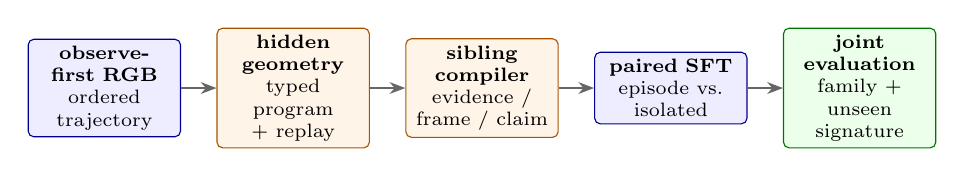
\begin{tikzpicture}[
      font=\scriptsize,
      box/.style={draw, rounded corners=2pt, align=center, minimum height=9mm,
                  text width=.145\linewidth, inner sep=2.5pt},
      visible/.style={box, fill=blue!7, draw=blue!55!black},
      hidden/.style={box, fill=orange!9, draw=orange!65!black},
      eval/.style={box, fill=green!8, draw=green!45!black},
      flow/.style={-{Stealth[length=2mm]}, semithick, draw=black!60},
      node distance=4.5mm]
    \node[visible] (acq) {\textbf{observe-first RGB}\\ordered trajectory};
    \node[hidden, right=of acq] (cert) {\textbf{hidden geometry}\\typed program + replay};
    \node[hidden, right=of cert] (family) {\textbf{sibling compiler}\\evidence / frame / claim};
    \node[visible, right=of family] (train) {\textbf{paired SFT}\\episode vs. isolated};
    \node[eval, right=of train] (test) {\textbf{joint evaluation}\\family + unseen signature};
    \draw[flow] (acq) -- (cert);
    \draw[flow] (cert) -- (family);
    \draw[flow] (family) -- (train);
    \draw[flow] (train) -- (test);
  \end{tikzpicture}
  \caption{\textbf{EpiSpace in one example and one pipeline.}
  The upper row shows a real evidence family: every input contains the same
  first RGB and one matched replacement; the answer to ``is there a piano?''
  must track the decisive view rather than the scene or language prior.
  Orange objects below are construction-only: pose, depth, masks, programs,
  and certificates never enter the student prompt.  Blue is the RGB--language
  interface; green denotes joint rather than independent-answer evaluation.}
  \label{fig:overview}
\end{figure}


An isolated sample $(O,q,y)$ does not identify that computation.  A model may
integrate the ordered observations $O$ into a reusable belief and execute the
query $q$, or map local image--language cues directly to $y$.  Answer loss
rewards both.  A fluent rationale does not establish that its intermediate
claims were correct or causally used.  Explicit maps, tools, simulator QA, and
streaming-memory benchmarks already provide valuable alternatives
\citep{sprite2026,s3bench2026,cog3dmap2026,sagent2026}; our goal is therefore
not to claim another first instance of any one component.  We instead seek a
controlled data intervention that tests evidence-sensitive compositional
behavior hidden by independent-answer accuracy.  Such behavior is necessary
for, but does not by itself identify, a reusable internal scene model.

Our first-principles unit is a \emph{counterfactual episode family}.  The
scene and latent fact are fixed across sibling records, while one legal
intervention changes the available evidence, the queried frame, or the truth
of a claim.  A complete evidence family contains (i) a matched prefix lacking
the decisive visual evidence, (ii) a revealed sibling containing it, and
(iii) a sibling in which that evidence is replaced; the answer must follow
\emph{unknown $\rightarrow$ known $\rightarrow$ unknown}.  Frame siblings
hold the two RGB images fixed while changing which camera defines forward, so
the categorical direction must transform.  Claim siblings use the same
cross-view geometry but balance true and false propositions.  These
obligations make evidence sensitivity measurable and expose the always-guess
and always-abstain solutions.

We combine families with an \emph{observe-first, read-many} training format.
An ordered RGB stream is presented before any downstream question, after
which up to six heterogeneous reads share that observation.  The model-visible
interface remains ordinary RGB and language.  A paired isolated-QA arm is
compiled from the identical fact and image set.  We provide two explicit
comparison regimes: fact matching quantifies serialized-input amortization,
whereas an importance-weighted schedule equalizes image occurrences and pixel
exposure.  The latter is a visual-exposure control, not a match of total text
tokens, training FLOPs, or wall-clock compute; these are reported separately.

\textbf{EpiSpace} realizes this design as a read-only compiler over
OmniGibson/BEHAVIOR-1K acquisitions~\citep{li2024behavior}.  It extracts raw
RGB from sensor archives; rejects trajectory--question mismatches; resolves
entity references with instance masks and a minimum-pixel rule; builds an
observable anchor-camera belief containing only seen entities; and attaches a
typed, answer-free program over grounding, frame, belief, metric, relation,
perspective, and verification operations.  Programs, poses, depth, masks, and
certificates never enter the primary prompt.  Each target is independently
recomputed from the source bundle, and a target render used for perspective
verification is excluded by both path and RGB hash.

The frozen pilot turns \EpiPlannedJobs{} planned jobs into
\EpiStrictBundles{} strict bundles over \EpiScenes{} scenes.  It contains
\EpiSourceViews{} model-visible RGB views, \EpiCompiledQuestions{} replayed
questions, and \EpiConsistencyFamilies{} complete sibling families.  The
paired train export supervises \EpiSupervisedFacts{} facts; the core benchmark
contains \EpiCoreBenchmarkRecords{} records, including
\EpiFamilyBenchmarkGroups{} scene-disjoint families and
\EpiCompositionRecords{} instances of two semantic program signatures absent
from training although every constituent operation is seen.

Our contributions are:
\begin{itemize}
  \item \textbf{A falsifiable supervision unit.}  Counterfactual evidence,
        frame, and claim siblings turn persistence, transformation, and
        epistemic honesty into joint obligations rather than independent QA.
  \item \textbf{A fail-closed geometry-to-episode compiler.}  Exact-input
        certificates, raw-channel isolation, typed hidden programs,
        reference-resolution gates, scene/family locks, and independent target
        replay produce auditable RGB--language records without exposing an
        oracle scaffold to the student.
  \item \textbf{A controlled benchmark and training contract.}  Same-fact and
        image-occurrence/pixel-matched schedules control facts and visual
        exposure while logging unmatched text/FLOPs; semantic-signature holdout tests
        composition; accuracy-conditioned evidence sensitivity prevents
        consistent-but-wrong behavior from appearing successful.
\end{itemize}

This submission reports the frozen data asset, its independent corpus audit,
and deterministic comparison schedules.  Model-training, external-transfer,
and human-evaluation results are intentionally outside the present evidence
and are not claimed.

\section{Related Work}
\label{sec:related}

\paragraph{Spatial supervision and evaluation.}
SpatialVLM scales metric supervision from reconstructed 3D cues
\citep{chen2024spatialvlm}; SenseNova-SI scales to eight million examples and
studies shortcuts and spatial chain-of-thought recipes
\citep{cai2025sensenova}.  VSI-Bench tests scene-walkthrough recall
\citep{yang2024thinking}; MindCube probes sparse-view mental simulation
\citep{yin2025mindcube}; MMSI-Bench diagnoses multi-image errors
\citep{yang2025mmsi}; and ViewSpatial-Bench varies the queried frame
\citep{li2025viewspatial}.  ReVSI audits answerability for the exact frames
shown \citep{revsi2026}, while ViewDiag shows that cross-view agreement can
coexist with geometric error \citep{viewdiag2026}.  MultihopSpatial evaluates
grounded 1--3-hop compositions, releases training data, and reports
reinforcement-learning transfer \citep{lee2026multihopspatial}.  We therefore
claim neither the first compositional spatial benchmark nor the first training
corpus; instead, exact-input certification and evidence-sensitive family
metrics are required here.

\paragraph{Systematic-composition protocols.}
CLOSURE tests known linguistic constructs in novel CLEVR contexts and finds
that even ground-truth programs need not ensure systematicity
\citep{bahdanau2019closure}.  CFQ formalizes atoms and compounds and controls
their train--test divergence \citep{keysers2020measuring}.  Our split follows
this tradition but is not CFQ/MCD: it only enforces seen typed atoms and
selected unseen program signatures in scene-disjoint multi-view episodes.

\paragraph{Programmatic and episodic data.}
SPRITE generates simulator-grounded QA with executable, metadata-checked
programs at scale \citep{sprite2026}.  S3-Bench studies streaming trajectories
and active exploration \citep{s3bench2026}; SpaMEM studies dynamic belief
updates \citep{spamem2026}; and EMemBench generates verifiable questions from
game trajectories \citep{emembench2026}.  Thus we claim no first simulator QA
generator, executable program, or trajectory benchmark.  MindEdit-Bench also
already studies physical counterfactuals that translate or rotate an object
\citep{yu2026mindedit}.  EpiSpace does not edit scene geometry: its
\emph{intervention sibling families} vary available evidence, the queried
reference frame, or the proposition being verified.  We use
\emph{counterfactual} only in this input-intervention sense.

\paragraph{Spatial maps, memories, and tools.}
Cog3DMap learns explicit 3D memory \citep{cog3dmap2026}; S-Agent accumulates
memory through spatial tools \citep{sagent2026}; OmniView-Space distills
query-aligned cognitive maps \citep{li2026omniview}; and Theory of Space probes
active belief construction \citep{theoryspace2026}.  EpiSpace claims none of
these mechanisms.  Its student receives RGB and language; simulator state and
typed programs are hidden construction certificates.  As in Visual Program
Distillation \citep{hu2023vpd}, executed structure supplies supervision without
requiring program emission or geometry tools at inference.

\paragraph{Precise scope of the contribution.}
EpiSpace combines four controls: certified intervention families;
an atom-seen, signature-unseen split; a fact- and image/pixel-exposure-matched
comparison of isolated QA with \emph{observe-first, read-many} training; and
accuracy-conditioned evidence sensitivity.  No component is claimed as a
first.  Together they test an episode-organization hypothesis under matched
facts and image/pixel exposure; total-token/FLOP matching remains a required
ablation.

\section{A First-Principles Learning Contract}
\label{sec:principles}

\paragraph{Why isolated answer supervision is insufficient.}
Let $O_{1:M}$ be an ordered observation stream and $q_k$ one of several
possible spatial reads.  Isolated SFT minimizes
$-\log p_\theta(y_k\mid O_{1:M},q_k)$.  This objective assigns equal reward to
a reusable write--read solution
\begin{equation}
  S_M=W_\theta(O_{1:M}), \qquad
  \hat y_k=R_\theta(S_M,q_k),
  \label{eq:write-read}
\end{equation}
and to query-specific functions
$\hat y_k=H_{\theta,k}(O_{1:M},q_k)$.  More paraphrases do not remove this
non-identifiability; a text rationale may itself be another unverified target.
Our contract changes both the presentation of evidence and the relations among
targets.

\paragraph{Observe first, then read many.}
In the episode arm, all RGB observations precede a batch of at most six
heterogeneous questions.  This causal serialization withholds questions until
after the visual tokens and prevents question-dependent selection of which
images are supplied; it does not establish query-independent perception or an
internal map.  A single observation set can support grounding, memory,
relation, metric, perspective, and verification reads.  The isolated arm
contains the identical selected facts and the same per-fact view sets but
repeats the observation for each question.  Fact matching and visual-exposure
matching are intentionally distinct: the former quantifies presentation
amortization; the latter uses a logged sampler and inverse-repeat loss weights
to equalize image and pixel occurrences, not total tokens or FLOPs.

\paragraph{Families turn evidence into an intervention.}
For a latent fact $z_f$, a family contains siblings
$\{(O_f^{(v)},q_f^{(v)},y_f^{(v)})\}_{v\in\mathcal V_f}$ generated by legal
interventions $I_v$.  The pilot materializes three obligation types.
\begin{itemize}
  \item \textbf{Evidence triples} share the question and image count.  Two
        context images are held fixed for cross-view triples (one for presence
        triples); replacing only the decisive image changes
        unknown$\rightarrow$known$\rightarrow$unknown.
  \item \textbf{Frame pairs} share exactly the same two RGB images and entity
        pair.  Only the camera declared as the forward frame changes; the
        relation label must transform accordingly.
  \item \textbf{Claim pairs} share the reconstructed cross-view relation while
        balancing a contradicted and a geometrically correct proposition.
\end{itemize}
Every sibling shares one consistency and split identifier.  A family is
discarded if a required member, unique reference, or matched-input obligation
cannot be certified.

\paragraph{Accuracy-conditioned evidence sensitivity.}
Let $c_{f,v}\in\{0,1\}$ indicate atomic correctness.  Family exact match is
$\prod_{v\in\mathcal V_f}c_{f,v}$.  For evidence triples with prefix $p$,
reveal $r$, and deletion $d$, we report reveal accuracy separately and
\begin{equation}
  \mathrm{ES}_{\mathrm{correct}}=
  \frac{\sum_f c_{f,r}c_{f,p}c_{f,d}}
       {\sum_f c_{f,r}},
  \label{eq:evidence-sensitivity}
\end{equation}
with an undefined denominator reported as N/A, never as a perfect score.
Always abstaining makes $c_{f,r}=0$ and therefore cannot score; always guessing
fails the two unknown siblings.  Frame-pair and claim-pair exact match are
reported separately.  Confidence intervals resample scenes, not nominal QA
rows.

\paragraph{A safe canonical observable belief.}
The compiler may construct $S_M$ as auxiliary supervision, but never exposes
omniscient world state.  Its origin is the ground projection of the first
camera; $+X$ is camera right, $+Y$ horizontal forward, and $+Z$ gravity up.
For entities visible in at least one input frame, it stores a Chinese category,
0.5\,m-quantized center and extent, first/last evidence views, and a
\texttt{visible} or \texttt{seen\_not\_current} status.  Never-observed entities
are excluded.  This state is a separately requested auxiliary target, not an
input to ordinary QA.  The pilot serializes terminal $S_M$ rather than a
per-view update sequence $\Delta S_{1:M}$; it therefore neither supervises
incremental state transitions nor demonstrates persistent internal memory.

\paragraph{Typed operations define, but do not reveal, composition.}
Each question is normalized to a directed acyclic program over grounding $G$,
frame alignment $F$, belief update $B$, metric estimation $M$, relation $R$,
perspective $P$, and verification $V$.  Node inputs and outputs are typed; the
IR contains no answer value and remains hidden.  The split withholds the full
signatures \texttt{counterfactual\_cross\_view.v1} and
\texttt{target\_view\_prediction.v1}, while all seven atoms occur in training
inside other programs.  Thus this narrow two-signature pilot tests new
compositions of seen operations on unseen scenes, not unseen operation tokens.

\begin{table}[t]
\centering
\small
\caption{Channel isolation.  Only the first row is used by primary SFT and
benchmark inference.}
\label{tab:contract}
\begin{tabular}{p{0.19\linewidth}p{0.31\linewidth}p{0.38\linewidth}}
\toprule
Channel & Contents & Function \\
\midrule
Model-visible & ordered raw RGB, camera height/FOV, natural language & ordinary
multimodal reasoning; no pose, depth, IDs, program, or target render \\
Supervision-only & observable belief, typed answer-free program & optional
state target, legality audit, signature label \\
Oracle-only & pose, metric depth, instance masks, world geometry, certificate &
deterministic construction, margins, replay, held-out verification \\
\bottomrule
\end{tabular}
\end{table}

\section{The EpiSpace Data Engine}
\label{sec:engine}

\subsection{Acquisition contract and raw-channel isolation}

EpiSpace consumes existing OmniGibson acquisition bundles without mutating
them.  Each bundle contains a trajectory plan, ordered observations, camera
transforms, an entity inventory, RGB/depth/instance sensor arrays, and quality
reports.  The sweep plan is the authoritative job ledger.  The frozen policy
accepts only jobs marked \texttt{passed}; the adapter additionally requires all
core files, contiguous view indices, non-empty entities, integrity
\texttt{pass}, and a compatible trajectory class.  Review and failed jobs are
preserved in a reason-coded ledger.

Human previews concatenate RGB, depth, and instance-ID panels and are therefore
forbidden as model input.  The loader extracts the \texttt{uint8} RGB array from
each sensor archive into a release-owned PNG, records its dimensions and raw
pixel SHA-256, and stores instance pixel counts in a sidecar used only during
compilation.  A purity gate decodes every referenced image, verifies
1024$\times$1024 RGB content against the sidecar, and rejects paths under a
preview directory.  Target-view renders are checked against all SFT inputs by
both path and decoded RGB hash.

Across seven sweeps, \EpiPlannedJobs{} planned jobs produce
\EpiStrictBundles{} strict bundles.  Of these, \EpiSourceTrajectories{} are
write sources with \EpiSourceViews{} raw RGB views; 21 T10 bundles are verifier
sources only.  A fixed hash ranking assigns all descendants of each scene to
32/7/7 train/validation/test scenes.  No trajectory, sibling family, or target
render crosses that boundary.

\input{generated/dataset_table}

\subsection{Trajectory semantics and question legality}

Camera motion determines which supervision is identifiable.
\begin{itemize}
  \item \textbf{T1 walkthroughs} support overlap, revisit, separated-view
        registration, memory, metric, relation, and perspective reads.
  \item \textbf{T3 rotation stations} change yaw at a fixed position.  We
        supervise two-frame change detection only when exactly one eligible
        object enters view; metric tasks are rejected because rotation adds no
        translational baseline.
  \item \textbf{T4 adaptive arcs} keep a focus instance visible across a
        collision-free partial orbit.  The safe target is observed-instance
        identity, not canonical front or an unseen backside; these uniformly
        positive items are training-only.
  \item \textbf{T7 elevation ladders} change height and pitch at a station.
        Two sufficiently visible, unique objects are compared in an explicitly
        declared anchor-camera frame.
  \item \textbf{T8 reveal paths} provide a decisive category-presence view and
        matched evidence-deletion controls when such a family is valid.
  \item \textbf{T10 target views} never enter a write prefix.  Their RGB is an
        oracle-only observation used to grade visibility predicted from a
        same-scene write trajectory.
\end{itemize}
T2, T5, T6, and T9 remain expansion slots and are not counted as pilot assets.

Source questions must have an accepted/unknown status, a terminal source
certificate, and evidence views inside the actual model sequence.  Instance
questions are retained only when category-plus-view resolves one entity and at
least one declared anchor contributes 500 instance pixels.  T10 origin,
facing, and candidate entities require their own unique observed anchors.
Direction surfaces explicitly name the frame.  All 241 observed ontology
categories are deterministically localized into Chinese; an audit searches
model-visible text for residual raw labels.

\subsection{Geometry first, language second}

The compiler fixes an entity binding and structured target before realizing a
question.  Relations are computed in the declared camera frame; distances are
rounded only after metric evaluation; last-seen labels are recomputed over the
actual presented view list; and unknown means that the required category or
referent is absent from those inputs, not absent from simulator world truth.
Natural-language templates then verbalize the fixed target.  This ordering
prevents a data-generation paraphraser from defining label geometry or reading
the answer-side certificate; it does not prevent a trained student from making
geometric errors.  Future paraphrasers must consume only question-side facts
and remain answer-blind.

Each accepted item receives a globally unique fact ID, exact model/evidence
views, entity IDs in hidden metadata, a typed program, a Chinese surface
answer, and a replay certificate.  The independent replayer does not trust a
stored \texttt{passed} bit: it loads the source bundle and recomputes the target
for all 17 task/program types.  The frozen release replays
\EpiReplayedCertificates{}/\EpiReplayedCertificates{} targets successfully.

\subsection{Counterfactual family compiler}

The generic family compiler expands validated atomic facts rather than relying
only on rare hand-authored trajectories.
\begin{itemize}
  \item \textbf{Presence evidence (85 triples):} one background RGB is shared
        by all siblings; the second RGB is either a category-free distractor,
        a $\geq500$-pixel decisive view, or a different distractor.
  \item \textbf{Cross-view evidence (5 triples):} two RGBs, including the
        canonical anchor and one resolvable referent, are shared; only the
        third image reveals or withholds the second never-co-visible referent.
  \item \textbf{Trajectory reveal (1 triple):} a T8 decisive view is exchanged
        against a matched category-free view.
  \item \textbf{Frame equivariance (\EpiFrameFamilies{} pairs):} the same two
        images and objects are retained, but forward is anchored to image one
        versus image two; only pairs whose oracle relation changes are kept.
  \item \textbf{Claim verification (\EpiClaimFamilies{} pairs):} each certified
        cross-view relation yields balanced true and false claims with a
        structured corrected relation.
\end{itemize}
This produces \EpiConsistencyFamilies{} complete families.  Missing siblings,
unequal image counts, inconsistent family IDs, and cross-split membership are
release-blocking errors.

\subsection{Exports and fail-closed validation}

One intermediate episode IR is rendered into observe-first SFT, paired
isolated SFT, optional observable-state SFT, RLVR-ready prompts, and benchmark
rows.  The full diagnostic benchmark contains \EpiBenchmarkRecords{} records.
The recommended core is the union of all scene-disjoint family rows and all
semantic-signature holdouts: \EpiCoreBenchmarkRecords{} unique rows, with
separate \texttt{family} and \texttt{composition} views for disaggregated
reporting.

Eighteen release gates cover program typing; atom-seen/signature-unseen
composition; scene and family locks; complete sibling shapes; shared family
IDs; identical episode/isolated fact multisets; globally unique fact and record
IDs; target-view path and hash isolation; raw-RGB purity; functional
input--target dependence; terminal certificates; passing certificate checks;
and full independent replay.  All pass.  The manifest also retains
\EpiRejectedItems{} exclusions, dominated by ambiguous references, failed or
review acquisition jobs, trajectory-illegal tasks, small referents, and
verifier-only bundles.  Exclusions are part of the reported yield rather than
silently discarded data.

\section{Learning and Evaluation Interfaces}
\label{sec:training}

The student is never trained to print the hidden operation graph.  All primary
records use a Qwen-compatible multimodal chat schema: raw RGB and Chinese text
are user content, and loss is applied only to assistant tokens.  Hard spatial
reads receive a short evidence-grounded explanation ending in the surface
answer; simple presence and metric reads use the answer directly.

\paragraph{B: observe-first episode SFT.}
For each selected view set, the user first supplies all ordered images and then
a numbered batch of at most six questions.  The assistant returns aligned
numbered answers.  The frozen train arm contains \EpiEpisodeRecords{} records
covering \EpiSupervisedFacts{} facts.  A whole-turn token mean would silently
give long answers and multi-question records different mass.  We instead map
each numbered answer to an exact tokenizer span.  For fact $f$ in record $i$,
let
\(
\ell_{if}=-|T_{if}|^{-1}\sum_{t\in T_{if}}
\log p_\theta(x_{it}\mid x_{i,<t},O_i)
\).
With schedule weight $w_i$, the implemented objective is
\begin{equation}
  \mathcal L_B(\theta)=\frac{1}{|\mathcal F|}
  \sum_i w_i\sum_{f\in\mathcal F_i}\ell_{if}.
  \label{eq:sft}
\end{equation}
Numbering, system, user, image-placeholder, program, and certificate tokens
have zero loss.  Under the repeated-record schedule below, this makes every
selected fact's total epoch weight exactly one.

\paragraph{Comparison groups are optimizer units.}
For the visual-exposure-controlled schedule, rows are partitioned by
\texttt{comparison\_id}.  For each $k$-fact group, either $k$ weighted episode
draws or $k$ one-fact isolated draws are backpropagated before exactly one Adam
update.  Both arms must pass paired group/fact/draw validation and use the same
seeded group order.  Per-draw Adam stepping is ineligible because inverse-repeat
weights do not commute with Adam (Appendix~\ref{app:matching}).

\paragraph{C: paired isolated-QA control.}
Each selected fact is separately exported over the same view list, yielding
\EpiIsolatedRecords{} records.  A comparison ID links each isolated row to its
episode record; explicit fact IDs verify equality of the fact multisets.  The
fact-matched regime measures serialized-input amortization (1,168 versus 3,227
image presentations), not runtime efficiency.  The stricter regime matches 651
draws, 3,227 image occurrences, and 3,383,754,752 pixels per arm through
inverse-repeat weights.  Exact profiling gives equal image tokens but 14.70\%
more total input tokens for episodes; neither regime matches total tokens,
training FLOPs, or wall time (Appendix~\ref{app:matching}).

\paragraph{Optional interfaces.}
Arm D contains \EpiStateRecords{} separately requested terminal-belief targets;
it is never a hint inside B/C and is tested only after their comparison.
Another \EpiRLVRRecords{} rows carry hidden, deterministic reward
specifications.  They are verifier-ready; no state-auxiliary, GRPO, policy, or
family-reward result is claimed.

\paragraph{Core benchmark protocol.}
The \EpiCoreBenchmarkRecords{}-row core de-duplicates
\EpiFamilyBenchmarkRecords{} family and \EpiCompositionRecords{} signature
rows.  It reports structured atomic, evidence, claim, frame, and
Eq.~\ref{eq:evidence-sensitivity} metrics.  Family exact match is restricted to
the \EpiFamilyBenchmarkGroups{} complete sibling consistency groups; canonical
composition-only rows are excluded.  Target-copy predictions validate wiring,
not model capability.

\paragraph{Falsifiable model study.}
The future full study trains the same 8B initialization under B/C with the same
optimizer, replay, group order, and updates.  Its primary outcome is
macro-averaged test accuracy on the two held-out signatures; 18 validation and
nine test rows are never pooled for a primary claim.  Family metrics are
co-primary and uncertainty clusters by scene/family.  A positive result still
requires total-token/FLOP matching before attribution to organization alone.

\section{Data-Asset Validation}
\label{sec:experiments}

We measure the frozen corpus, schedules, and evaluator; target-copy predictions
test wiring and are not a spatial-reasoning baseline.  No trained-model result
is reported here.

\subsection{Frozen pilot yield}

Of 322 terminated jobs, fail-closed loading retains 172 write trajectories and
21 T10 verifiers over 46 scenes: 1,063 RGB views compile into 1,093 questions.
The export has 340 episode, 651 isolated, 116 optional-state, and 651
verifier-ready rows.  All 133 groups have their required shape (91 evidence,
37 claim, five frame); exclusions remain reason-coded.

\subsection{Benchmark partitions and shortcut visibility}

The 370-row validation/test diagnostic contains a 112-row family view with 42
scene-disjoint sibling groups and a 27-row composition view (18 validation,
nine test); their union is the 115-row core.  A same-partition target-majority
diagnostic reaches 62.61\% on the core but is neither learned nor no-image.
Target-copy recovers 115/115 rows, 42 sibling groups, 28 evidence triples
(14/14 validation/test), 12 claim pairs, and two validation-only frame pairs.
Canonical composition-only rows never count as families; malformed or missing
predictions are incorrect.

\subsection{Independent integrity evidence}

Geometry replay and an implementation-independent serialized audit reproduce
1,093/1,093 targets and all 133 shapes, find no split leakage or raw ontology in
20,503 visible text fields, and verify paired facts, held-out signatures,
target-view hash isolation, and input--target functionality.  The eighteen
gates and portability boundary are in Appendix~\ref{app:gates}.

\subsection{Facts and visual exposure are separate controls}

Fact matching yields 63.81\% fewer serialized image presentations, not measured
runtime savings.  The stricter schedule matches facts, draws, images, pixels,
and optimizer groups, but episodes retain 14.70\% more total input tokens;
FLOPs and wall time remain unmatched (Appendix~\ref{app:matching}).  These
controls imply no learning gain; the frozen comparison remains to be reported.

\section{Conclusion}
\label{sec:conclusion}

EpiSpace turns spatial episode learning into a controlled behavioral test through the
conjunction of geometry-replayed intervention families, an
atom-seen/signature-unseen split, and fact- and image/pixel-exposure-controlled
episode versus isolated schedules.  Its pilot provides 1,093 certified
questions, 133 families, 651 paired facts, and a 115-row core.  Every target
replays from source geometry while prompts contain only RGB and language.  This
validates the asset and evaluator, not a learned representation; the matched
training comparison remains decisive.

\paragraph{Limitations.}
This 46-scene, mostly static pilot lacks interaction, real-camera shift, and
human calibration.  Presence dominates evidence triples (85/91); the
composition partition has only 18 validation and nine test rows, and no frame
pair lies in test.  Templates limit language breadth, and unknown priors require
joint metrics.  The optional belief is a terminal target, not per-view
$\Delta S$ supervision or evidence of a learned internal state.  Local media
paths and source terms limit portability; corpus checks establish neither
learning, RLVR, nor external transfer.


\bibliography{references}
\bibliographystyle{iclr2026_conference}

\appendix
\section{Serialized Data Contracts}
\label{app:schemas}

All files are UTF-8 JSONL except manifests and reports, which are JSON.  Table
\ref{tab:schemas} lists the minimum public contract; additional hidden fields
retain provenance and permit audits.

\begin{table}[h]
\centering
\small
\caption{Principal serialized artifacts.}
\label{tab:schemas}
\begin{tabular}{p{0.28\linewidth}p{0.64\linewidth}}
\toprule
Artifact & Required content \\
\midrule
\texttt{episodes.ir.jsonl} & episode/scene/trajectory IDs, split lock, ordered
observations, observable belief, and question list \\
\texttt{train.episode\_sft.jsonl} & messages, assistant-only loss policy, and
comparison contract for an observe-first question batch \\
\texttt{train.isolated\_sft.jsonl} & one paired fact per dialogue with the
same evidence views and comparison ID \\
\texttt{train.state\_aux\_sft.jsonl} & separately requested observable-state
target; never inserted into primary QA \\
\texttt{train.rlvr.jsonl} & prompt and hidden deterministic reward specification;
no claim that policy training was run \\
\texttt{benchmark*.jsonl} & record/family/scene IDs, split, model input,
structured target, hidden program, certificate, and evidence provenance \\
\bottomrule
\end{tabular}
\end{table}

An IR observation is
\texttt{\{view\_id, step, role, rgb\}}.  A question stores
\texttt{fact\_id}, task, Chinese surface question/answer, structured answer
value/status, program, model/evidence view IDs, family variant, and certificate.
The answer-free program contains a semantic signature, typed atoms and nodes,
external inputs, and one answer node.  The certificate contains named checks,
oracle-only replay inputs, terminal result, and verifier version.  Programs,
certificates, entity IDs, pose, depth, and masks are excluded from ordinary
model messages.

Episode and isolated records share a \texttt{comparison\_id}; their comparison
contracts declare fact IDs, unique-image count, question count, and arm.  The
minimal prediction format is:
\begin{verbatim}
{"record_id":"benchmark-...","answer_value":<JSON value>}
\end{verbatim}
The evaluator requires exactly one prediction per benchmark record.  Strings,
booleans, nulls, lists, and dictionaries are compared with exact types and
keys; finite numeric fields use the tolerance stored in the certificate.

\section{Fail-Closed Gates}
\label{app:gates}

The release manifest records eighteen Boolean gates.  A failed gate makes the
build fail rather than merely attaching a warning:
\begin{enumerate}
  \item \texttt{typed\_programs\_valid},
        \texttt{heldout\_program\_absent\_from\_train}, and
        \texttt{heldout\_atoms\_seen\_in\_train};
  \item \texttt{scene\_split\_lock}, \texttt{family\_split\_lock},
        \texttt{family\_members\_complete}, and
        \texttt{family\_intervention\_contract};
  \item
        \texttt{family\_id\_shared\_within\_consistency\_group};
  \item \texttt{paired\_fact\_multiset\_equal},
        \texttt{fact\_ids\_globally\_unique}, and
        \texttt{record\_ids\_unique};
  \item \texttt{heldout\_target\_rgb\_absent\_from\_sft\_input},
        \texttt{heldout\_target\_rgb\_hash\_absent\_from\_sft\_input},
        \texttt{rgb\_channel\_purity}, and
        \texttt{normalized\_input\_functional\_dependency};
  \item \texttt{all\_certificates\_terminal},
        \texttt{all\_certificate\_checks\_pass}, and
        \texttt{certificate\_full\_reexecution}.
\end{enumerate}

The independent corpus audit is intentionally separate.  It parses every
serialized row, recomputes family shapes and cluster leakage, opens all image
paths, scans model-visible text for raw ontology tokens, measures target
priors, and compares episode/isolated facts and image exposure.  It never calls
the builder, compiler, exporter, or geometry verifier.  Without a prediction
file, model-dependent evidence sensitivity is reported as not evaluated.

\section{Metrics}
\label{app:metrics}

Let $c_i$ be structured exact correctness for record $i$.
\textbf{Atomic accuracy} is the mean of $c_i$, disaggregated by task, program,
and split.  For one of the 42 complete sibling consistency groups $f$,
\textbf{family exact match} is $\prod_{i\in f}c_i$.  Rows with no sibling
consistency group, including canonical target-view composition rows, are never
treated as singleton families.  Evidence-triple exact match and the conditioned score in
Eq.~\ref{eq:evidence-sensitivity} are both required: reveal accuracy is the
denominator, so an always-unknown model cannot receive evidence-sensitivity
credit.  \textbf{Claim-pair exact match} requires both true and false siblings.
\textbf{Frame equivariance} requires both same-RGB frame answers to match their
respective targets; merely changing between two wrong labels earns no credit.
\textbf{Composition accuracy} is atomic accuracy on the two held-out semantic
signatures and is always reported separately from family metrics.

Missing, duplicate, extra, malformed, or non-finite predictions are incorrect.
When model results are eventually produced, uncertainty is computed by
resampling the scene/family unit rather than treating sibling rows as
independent.  The same-partition task-majority number is labeled an oracle
diagnostic and is never presented as a trained no-image baseline.

\section{Matching Regimes}
\label{app:matching}

The fact-matched schedules require equality of the raw and effective fact
multisets.  They preserve the natural amortization difference: 340 episode
draws/1,168 image occurrences versus 651 isolated draws/3,227 occurrences.
The image-occurrence-matched schedules repeat an episode once per selected
fact and assign each repeat inverse multiplicity.  Required invariants are
equality of the effective fact-weight multiset, exact image-occurrence
multiset, and pixel exposure.  The resulting two arms each contain 651 draws,
3,227 image occurrences, and 3,383,754,752 pixels.  The manifest's text count
is only a Unicode-lexeme proxy.  A separate exact Qwen3-VL-4B profile at
$256^2$ reports 206,528 image tokens per arm but 415,424 versus 362,185 total
input tokens and 208,896 versus 155,657 text tokens (episode versus isolated).
Thus neither the fact-matched nor image-occurrence-matched regime is a
total-token, FLOP, or wall-clock-compute match.

The controlled optimizer unit is one \texttt{comparison\_id}, not one draw.
For a group of $k$ facts, the episode schedule contains $k$ identical $k$-fact
draws with weight $1/k$; its isolated counterpart contains $k$ distinct
one-fact draws with weight one.  The trainer zeros gradients once, accumulates
all $k$ draws, and calls Adam once.  It rejects unequal paired group IDs, fact
sets, draw counts, or update counts.  Stepping Adam after each weighted draw is
a legacy diagnostic, not a controlled comparison: Adam's nonlinear moments do
not make a $1/k$-scaled update equivalent to one grouped update.

\section{Reproduction Commands}
\label{app:commands}

Commands are run from the repository root with the project interpreter.
\begin{verbatim}
PY=../habitat/.conda/core/bin/python

$PY -m episode3d.cli \
  --config configs/epispace_pilot_v1.json

$PY scripts/build_compute_matched_schedules.py \
  --episode data/epispace_pilot_v1/train.episode_sft.jsonl \
  --isolated data/epispace_pilot_v1/train.isolated_sft.jsonl \
  --output-dir data/epispace_pilot_v1/compute_matching \
  --seed 17

$PY -m episode3d.corpus_audit \
  data/epispace_pilot_v1

$PY -m episode3d.benchmark_evaluator oracle \
  --benchmark data/epispace_pilot_v1/benchmark.core.jsonl \
  --output /tmp/epispace-oracle.jsonl

$PY -m episode3d.benchmark_evaluator evaluate \
  --benchmark data/epispace_pilot_v1/benchmark.core.jsonl \
  --predictions /tmp/epispace-oracle.jsonl \
  --output-dir /tmp/epispace-evaluation

$PY -m pytest -q
$PY -m ruff check episode3d scripts tests
\end{verbatim}

The oracle command copies structured targets solely for evaluator smoke
testing.  It must never be used as a model result.  The authoritative frozen
statistics are in \texttt{release\_manifest.json}; serialized-only diagnostics
are in \texttt{corpus\_audit.json}; schedule invariants and hashes are in
\texttt{compute\_matching/compute\_matching\_manifest.json}.

\section{Asset and License Boundaries}
\label{app:license}

Raw RGB PNGs are extracted into a release-owned cache, but current JSONL rows
store machine-local absolute paths.  Consumers must remap the cache prefix
without changing content hashes.  BEHAVIOR-1K-derived renders remain governed
by their source academic-use terms.  The present internal artifact does not
grant redistribution permission.  No real-world transfer, human calibration,
or model-training result is part of this frozen release.


\end{document}
